To investigate the issue of irreproducibility empirically, we built an experimental setup and a working pipeline. Consistency across runs should be maintained as much as
possible by using the same settings and established methods for control. By accounting for other sources of randomness,
we aim to isolate and document the impact of CUDA execution-related randomness. 
This will involve analyzing performance variance for patterns and correlations. The credibility of the results will be ensured by the correct isolation of the randomness.
we execute the multiple runs while carefully managing all sources of randomness. 
The exact number of runs is depend on factors such as GPU capabilities and environmental conditions, 
but we anticipated 180 independent runs overall. The reasoning for this number will be explained later in this chapter.

\section{Experiment Design and Objectives}
Our investigation revolves around the question of the influence of CUDA-induced randomness on the reproducibility and robustness of deep learning applications, specifically within the realm of computer vision. We have termed this central investigation as the Main Question (MQ):

\begin{quote}
\textbf{MQ:} \textit{What is the overarching impact of CUDA randomness on the reproducibility and performance of deep learning tasks in computer vision?}
\end{quote}

To dissect this question and gain a more granular understanding, we have broken it down into three specific sub-questions:

\begin{enumerate}
    \item Our first sub-question addresses the performance variation in deep learning tasks when we control for other potential sources of randomness but deliberately allow the inherent randomness from CUDA execution. The aim here is to gauge the degree to which CUDA randomness alone can influence the outcome. To this end, we execute five identical runs in each configurations to record the variance and ensure the reliability of our findings. This is encapsulated in:
    \begin{quote}
    \textbf{SQ1:} \textit{What is the extent of performance variability when controlling for other sources of randomness, while allowing for randomness from CUDA execution to be present?}
    \end{quote}

    \item The second sub-question explores the implications of using deterministic settings within CUDA. While deterministic approaches may provide reproducibility, they might come with their own set of trade-offs. By having deterministic CUDA execution in some configurations, we intend to shed light on any potential performance or computational costs associated with such an approach. This is summarized in:
    \begin{quote}
    \textbf{SQ2:} \textit{What is the cost of using deterministic approaches in CUDA randomness?}
    \end{quote}

    \item Lastly, our third sub-question addresses the practical implications of CUDA randomness in specific real-world domains. By utilizing two domain-specific datasets — one from Civil Engineering and the other from Medicine — we aim to unearth the nuances of how CUDA randomness might differentially affect performance and computation costs in these specialized areas. This practical aspect of our research is framed as:
    \begin{quote}
    \textbf{SQ3:} \textit{How does the randomness in Computer Vision impact the task performance and computation cost for specific applications, such as Civil Engineering and Medicine?}
    \end{quote}
\end{enumerate}

By investigating these sub-questions, we hope to provide a comprehensive answer to our main research query, bridging the gap between theoretical understanding and practical implications of CUDA randomness in computer vision-based deep learning tasks.\\

One main solution to reduce the randomness in deep learning applications is fixing the seeds.
Seeding is a fundamental practice in deep learning that allows the random number generator to produce same random numbers everytime. As mentioned, inherent randomness arises from, for example, initialization of weights, data shuffling, and data augmentation. This randomness can lead to variations in model performance and outcomes, even when the model is trained with the exact same parameters and data. By fixing the seed value, often referred to as "setting the seed", we can ensure up to some point that these random operations produce consistent results every time the model is run. This deterministic behavior is crucial when we wish to reproduce results, compare the efficacy of different models, or ensure consistent behavior across runs. 
For experiments, we think that different seed configurations might show different results and sensitivity
to CUDA-caused randomness. Thus, we have five different seed configurations and these are chosen randomly. \\

The strategy detailed above can be better understood through the experimental structure illustrated in the figure \ref{fig:runs_exp}.\\
      
\begin{figure}[htbp]
    \centerline{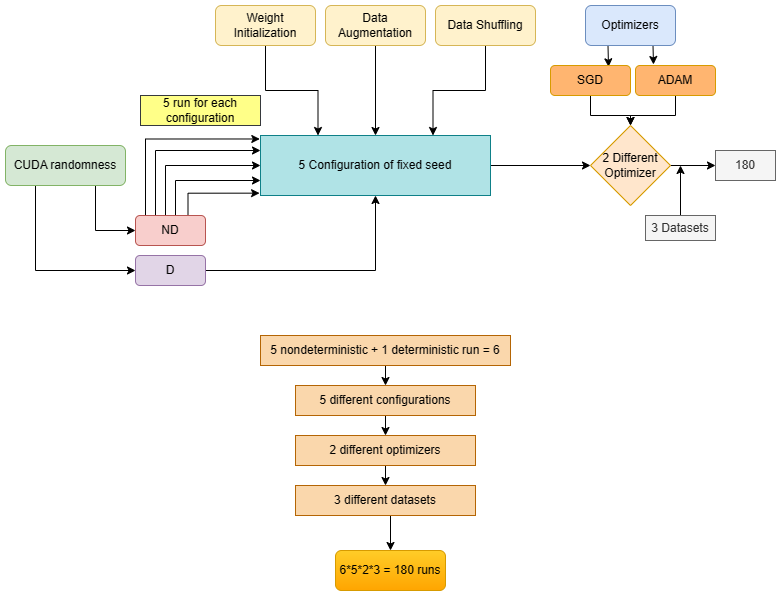
\includegraphics[scale=.5]{figures/runs.png}}
    \caption{Structure of the experimentation}
    \label{fig:runs_exp}
    \end{figure}
 
As can be seen from the figure \ref{fig:runs_exp}, there are \emph{two} options available for randomness settings in CUDA: nondeterministic and deterministic.
There are \emph{five} separate runs using fixed seed configurations
with nondeterministic CUDA settings while controlling all other sources of randomness. That means in the experiments,
framework, used libraries and versions, hardware and other environmental factors will be kept the same.
Additionally, we have \emph{one} run using deterministic CUDA settings.
Ultimetaly, We use \emph{two} commonly used optimizers to find out the optimizer influence and conduct the tests on \emph{three} different datasets,
resulting in a total of \emph{6*5*2*3 = 180}  runs.

\section{Datasets}

In this work, we use only publicly available sources. As a start, CIFAR-10~\cite{krizhevsky2009learning} dataset is used. Experiments on CIFAR-10 will 
provide neutral analysis that would represent the image classification tasks generally and help build the experimentation setup. Additionally,
two different datasets from two different domains will be taken into account. Investigating these two use cases will unlock the 
opportunity to answer the fourth question. 
We use SDNET2018~\cite{maguire2018sdnet2018} as the use case from Civil Engineering. There are several papers that for comparisons and validations. One example is the
work of Dorafshan et al.~\cite{dorafshan2018sdnet2018}.
The researchers showcased their crack detection algorithm's performance by conducting a series of tests using the aforementioned dataset.
The algorithm was developed based on the AlexNet Deep Convolutional Neural Network (DCNN) architecture~\cite{krizhevsky2017imagenet}, which enabled it to achieve accurate results. The dataset is publicly available and usable. 
In the Medical domain, the well-known breast cancer dataset CBIS-DDSM~\cite{spanhol2015dataset} is used.  
The choises of the datasets are made based on some criterias such as ease of applicability, availability, ease of implementation and the number of papers that use the dataset.
\\
\\
\subsection{Overview of the Datasets}

The CIFAR-10 dataset comprises 60,000 32x32 colour images categorized into 10 distinct classes. Each class encapsulates 6,000 images, aggregating to 50,000 training images and 10,000 testing images. The dataset is partitioned into five training sets and a singular testing set. Each training set contains 10,000 images, while the test set encompasses exactly 1,000 randomly chosen images from every category. The training sets exhibit a random order of images, with some sets potentially harboring a higher count of images from a particular category than others. However, cumulatively, the training sets possess an equal distribution with 5,000 images from each category. Table \ref{tab:Cifar-10 labels} delineates the labels within the dataset.\\

\begin{table}[h]
    \centering
    \begin{tabular}{ |c|c| }
        \hline
        Labels & Type \\
        \hline
         0 & Airplane \\
         1 & Automobile \\
         2 & Bird\\
         3 & Cat \\
         4 & Deer \\
         5 & Dog \\
         6 & Frog \\
         7 & Horse \\
         8 & Ship \\
         9 & Truck \\
        \hline
    \end{tabular}
    \caption{Labels in the CIFAR-10 Dataset}
    \label{tab:Cifar-10 labels}
\end{table}

Figure \ref{fig:cifar_10_eda} exhibits a selection of images from each class of the CIFAR-10 dataset, generated using a Python script. The figure elucidates the variability and characteristics inherent in each class, which is instrumental in understanding the complexity of the dataset. It's conspicuous that the dataset encapsulates a diverse range of features and attributes within each class, which underscores the necessity for robust machine learning models capable of discerning nuanced differences and similarities among the images.

\begin{figure}[h]
    \centering
    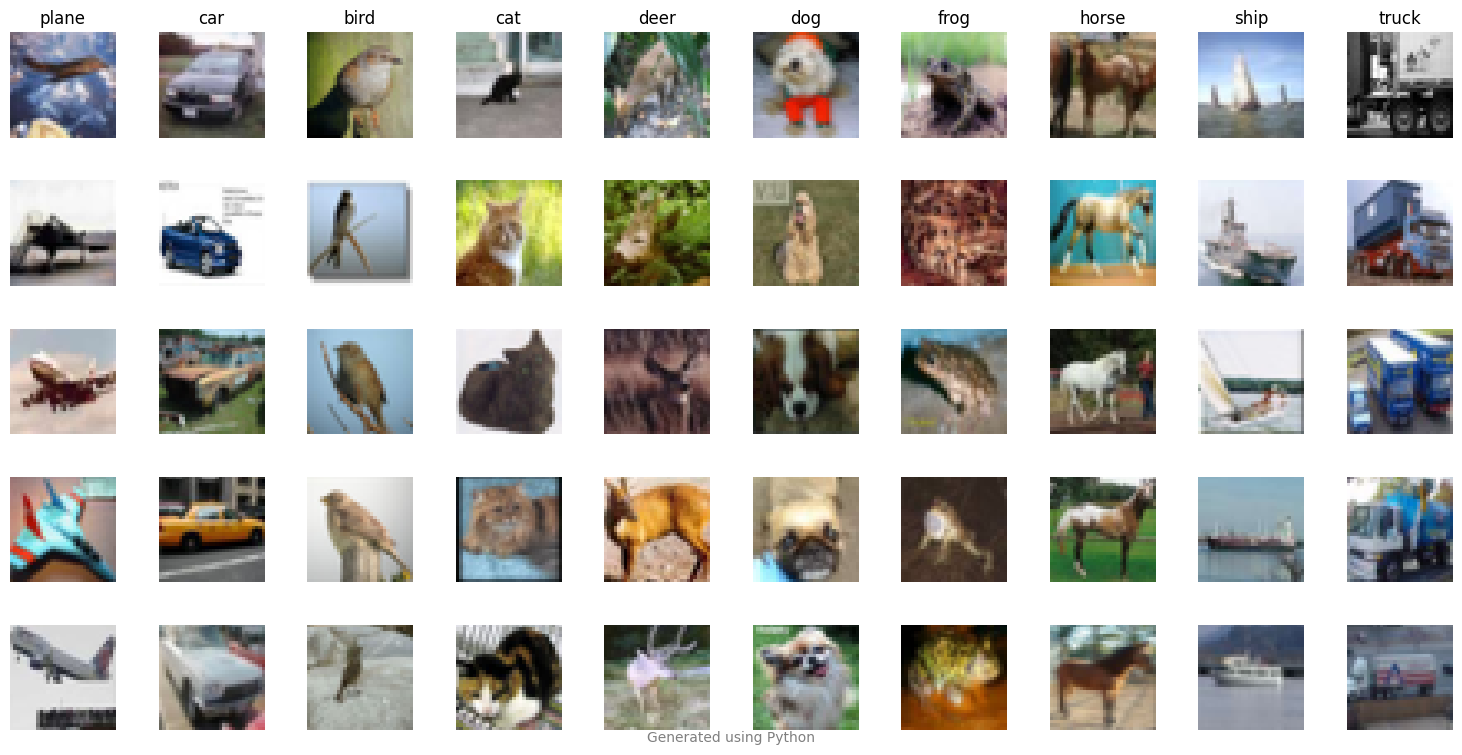
\includegraphics[width=0.8\textwidth]{figures/cifar_10_eda.png}
    \caption{Example images from each class of the CIFAR-10 dataset.}
    \label{fig:cifar_10_eda}
\end{figure}



The SDNET2018 dataset is a comprehensive collection of labeled images specifically designed to aid in the development and evaluation of AI algorithms for detecting cracks in concrete structures. Comprising over 56,000 images, this dataset provides a diverse representation of concrete structures, including walls, pavements, and bridge decks. These images capture both the presence and absence of cracks, with crack widths ranging from a minuscule 0.06mm to a prominent 25mm.\\

What makes SDNET2018 particularly valuable for training machine learning models is its inclusion of images that depict various real-world challenges. These challenges include obstructions such as shadows, surface roughness, scaling, edges, holes, and background debris. Such complexities make the task of automated crack detection more intricate, mirroring the actual challenges faced in real-world scenarios.\\

The ultimate goal of utilizing this dataset is to leverage machine learning and computer vision techniques to pinpoint and localize cracks across diverse structural backgrounds and amidst various obstructions. This is not just a technical challenge but also a matter of public safety. Accurate crack detection is pivotal for assessing the structural health of urban infrastructure, ensuring its longevity, safety, and cost-effective maintenance.\\

A glimpse into the SDNET2018 training set can be seen in Figure \ref{fig:output}, which was generated using a Python script. This figure highlights the varied conditions under which the AI algorithms are expected to operate. The labeled images in the dataset are categorized into two primary labels: "cracked" and "non-cracked". These images display a spectrum of crack appearances and obstructions, emphasizing the real-world intricacies of automated crack detection. Given the variability in crack width, orientation, and the presence of background interferences, there's a pressing need for the creation of robust algorithms. These algorithms should be adept at identifying even the most subtle structural discrepancies in a plethora of cluttered environments.\\

\begin{figure}[h]
    \centering
    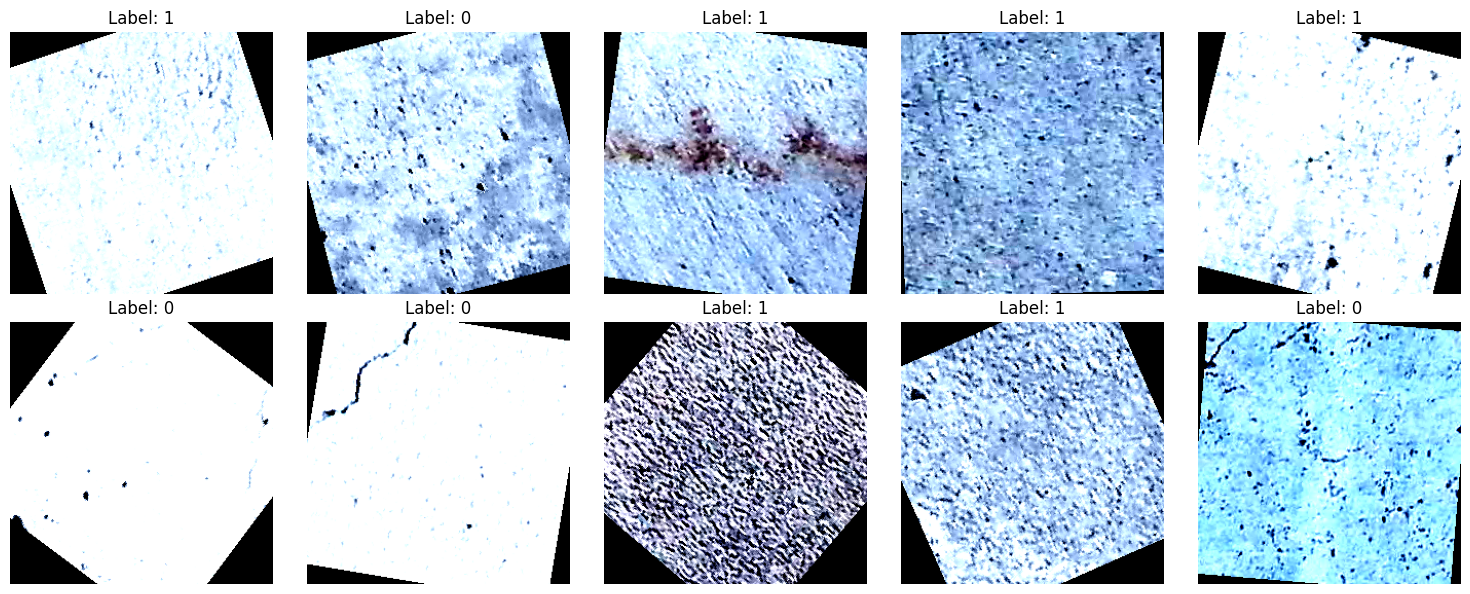
\includegraphics[width=0.8\textwidth]{figures/output.png}
    \caption{Random example images from the SDNET2018 training set with labels.}
    \label{fig:output}
\end{figure}

The CBIS-DDSM (Curated Breast Imaging Subset of DDSM) is a distinguished dataset in the domain of digital mammography research. It originates from the Digital Database for Screening Mammography (DDSM) and is curated to be more accessible for contemporary machine learning and computer vision applications.\\

The core of CBIS-DDSM is composed of mammographic images, encompassing both benign and malignant cases. The images are further categorized based on the type of lesion visible, such as masses or calcifications. The images in CBIS-DDSM have been converted to a more standard format to facilitate modern research, featuring improved lesion annotations and consistent metadata. Each image is accompanied by associated metadata, which may include the patient's age, the type of lesion, its location, and other relevant clinical details.\\

Due to its comprehensive nature and the diversity of cases it presents, the CBIS-DDSM has become an invaluable resource for researchers aiming to develop and validate breast cancer detection algorithms, especially those leveraging machine learning and computer vision.\\

The composition of the CBIS-DDSM dataset is detailed in Table \ref{tab:dataset-composition}, illustrating the distribution of images across different categories. The table segregates the images into benign and malignant cases, and further breaks down the data based on the type of lesions, i.e., masses and calcifications. It is evident from the table that the dataset provides a balanced representation of both benign and malignant cases, which is crucial for training machine learning models to recognize and differentiate between various types of lesions. Moreover, the distinct categorization of lesions into masses and calcifications aids in understanding the diverse nature of mammographic abnormalities present in the dataset, thereby enriching the scope of research in breast cancer detection.\\

% Table showing dataset composition
\begin{table}[h]
\centering
\caption{Composition of CBIS-DDSM Dataset}
\label{tab:dataset-composition}
\begin{tabular}{|l|c|}
\hline
\textbf{Category} & \textbf{Number of Images} \\
\hline
Benign & 1429 \\
Malignant & 1457 \\
Masses & 891 \\
Calcifications & 735 \\
\hline
\end{tabular}
\end{table}

Figure \ref{fig:breast_cancer} displays random example raw images from the CBIS-DDSM dataset, generated using a Python script. The images showcased serve as a stark reminder of the challenges inherent in mammographic image analysis. At a glance, it is difficult, especially for the untrained eye, to ascertain the precise location of cancerous lesions. The subtlety of mammographic abnormalities and the often-ambiguous nature of malignant versus benign indicators render the task of accurate identification and localization exceedingly challenging without substantial domain knowledge and expertise. Moreover, the visual similarity between benign and malignant lesions can further confound accurate classification, underscoring the necessity for sophisticated machine learning and computer vision algorithms capable of teasing apart these nuanced differences to aid in early and accurate breast cancer detection.

\begin{figure}[h]
    \centering
    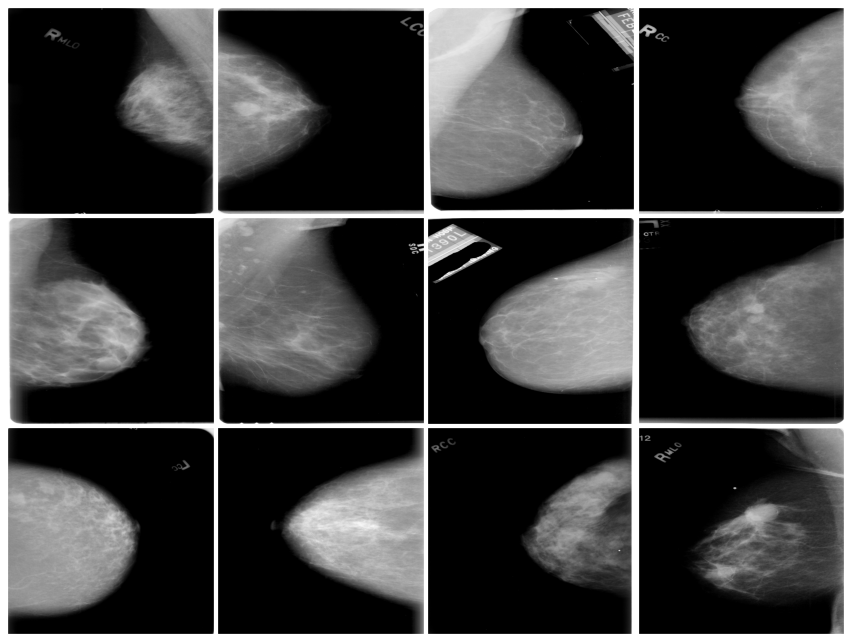
\includegraphics[width=0.8\textwidth]{figures/breast_cancer.png}
    \caption{Random example raw images from the CBIS-DDSM dataset.}
    \label{fig:breast_cancer}
\end{figure}


\section{Model Architectures}

The three tasks at hand involve classifying images and are of particular importance in the fields of civil engineering and medicine,
where they have real-world applications and deal with critical domains. In order to accurately represent real-world scenarios,
there is a strong inclination to achieve high performance on these tasks, which necessitates the use of recent and deep CNN~\cite{lecun1995convolutional} models. 
CNNs extract features from images through convolutional and pooling layers.
Convolutional layers apply filters to small regions of the image, producing feature maps that highlight patterns.
Pooling layers downsample the feature maps to reduce their dimensionality.
This hierarchical feature extraction enables CNNs to learn complex representations of the image, which can be used to classify the image into different categories.
It is important to use CNN models that are commonly used in the scientific community in order to ensure that the results can be validated.
However, hardware and time constraints must also be taken into consideration when selecting models for these tasks, as each run must complete 
in a reasonable amount of time to allow for the timely completion of the experiments. Ultimately, the choice of model will be based on these factors.\\

Three architectures used in this study are PreActResNet~\cite{DBLP:journals/corr/HeZR016}, ResNet~\cite{he2015deep} and MobileNet~\cite{DBLP:journals/corr/HowardZCKWWAA17}. These are used in CIFAR-10, CBIS-DDSM and SDNET datasets, respectively. Below is the short overview of these architectures:\\

\textbf{ResNet (Residual Network)}:
Introduced by Microsoft Research in 2015, ResNet brought the novel concept of "residual blocks" to tackle the vanishing gradient problem in deep networks. This innovation permits the training of considerably deeper networks by introducing shortcut or skip connections that bypass one or more layers. The architecture has several variants including ResNet-18, ResNet-34, ResNet-50, ResNet-101, and ResNet-152, where the numbers indicate the network's depth.\\

\textbf{PreActResNet}:
A variant of ResNet, PreActResNet employs pre-activation within its residual blocks, placing activation functions before weight layers, which has shown improved performance over the original design.\\

\textbf{MobileNet}:
Designed by Google, MobileNet is tailored for efficiency, making it suitable for devices with computational limitations, like mobiles. The architecture's defining feature is its use of depth-wise separable convolutions which substantially reduce the number of parameters, rendering the network lightweight and swift. MobileNet has seen several improvements with versions like MobileNetV1, MobileNetV2, and MobileNetV3, each refining the design to enhance efficiency.\\

The architectures for the three task at hand by chosen their usability, availability and implementation easiness as well as popularity in the community. Another aspect is the limitation of time and hardware. We see that for concrete crack detection we need robust and lightweight architectures as seen in the work of Zhang et al.~\cite{ZHANG2023131941}. Usage of ResNet architectures are so common there are lots of paper that uses these architectures for benchmarks.

\section{Experiment Pipeline}

Our experimental pipeline is based on the the \emph{HPC} infrastructure at IKIM, which is specifically optimized for the computational demands of deep learning. This robust setup ensures that extensive model training and evaluations are conducted seamlessly, harnessing the full potential of modern deep learning methods.\\

Resource allocation and task scheduling are handled by the \emph{SLURM} job scheduler. SLURM's design guarantees that each experiment's computing processes don't overlap with others, ensuring dedicated and consistent computational power. Within this managed environment, our experiments run on Python, primarily utilizing the PyTorch framework. This choice is driven by PyTorch's flexibility in model design, its efficient tensor computations, and its vast library of tools and functions that expedite the deep learning process.\\

Access to \emph{Data} is facilitated via the Network File System (NFS), known for its speed and reliability. During the model training phase, PyTorch dataloaders play a pivotal role by efficiently batching and loading data, optimizing the GPU utilization. To maintain transparency and facilitate analysis, all experimental metrics are logged systematically. Additionally, \emph{Weights \& Biases} (W\&B) provides a platform for real-time visualization and monitoring, giving a clear insight into model performance, convergence rates, and other vital metrics. This structured approach ensures our research remains rigorous, consistent, and informed, as will be shown in the subsequent figure.\\



\begin{figure}[htbp]
    \centerline{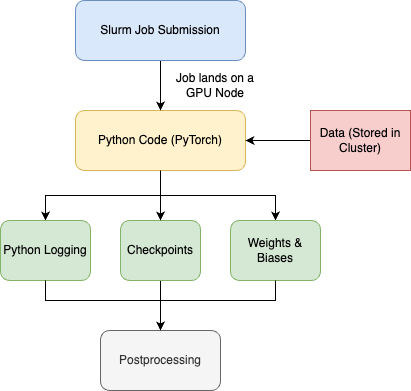
\includegraphics[scale=.5]{figures/Experiments_method.png}}
    \caption{Experiment pipeline}
    \label{fig:exp_pipeline}
\end{figure}


% todo: In-depth explanation of scientific method and how it is applied in our experiments. For example, every data augmentation or anything that is applied to increase the accuracy of the tasks should be mentioned here. Add also how similarities and variances calculated.

\section{Application of Certain Mathematical Methods}

Various mathematical methods have been employed as elucidated in the background chapter, each chosen for specific reasons to align with the objectives of this study. Below, the rationale behind the selection and application of each method is presented.\\

\textbf{Standard Variance:} 
Standard Variance is utilized to assess the dispersion in the outcomes and in the weight matrices, with particular attention to the variance within the last layer of the network. This focus is premised on the pivotal role the last layer plays in classification, embodying the cumulative contributions from all preceding layers. A component-wise standard variance is computed for each checkpoint, yielding a matrix mirroring the original in dimensions but encapsulating the variances in individual weights. The mean of this resultant matrix furnishes the standard variance for a specific configuration at a particular checkpoint. Replicating this process across all checkpoints and configurations facilitates a graphical representation, enabling insightful interpretations of the variance trends.\\

\textbf{Cosine Similarity:} 
Cosine similarity is employed to compare the weights of machine learning models in our study, following the approach of Fort et al. (2020), who utilized this metric for a similar purpose. Cosine similarity is a direct and intuitive measure, providing insight into how the weights diverge, particularly under the influence of CUDA-randomness, during training.\\

The method is applied to examine the similarity among weight matrices. However, a limitation arises as cosine similarity inherently facilitates pairwise comparisons, while our objective is to determine the mutual similarity across five separate runs. To address this, we compute pairwise similarity values for every possible pairing among the five runs, and subsequently average these values to derive a consolidated similarity metric for a given configuration. The procedure is as follows: similarities are computed between the first and second run, first and third run, and so forth, until the final pairing of fourth and fifth run. The mean of these values yields the aggregate similarity for the specific configuration. Further analysis entails extracting the mean, maximum, and minimum values from these computed similarities, which are then visualized to furnish a comprehensive overview of the similarity metrics across various configurations and checkpoints.\\

Referring to the visualizations below, for each distinct configuration, we construct a \(5 \times 5\) matrix showcasing similarity values. The indices within this matrix denote run pairs. By focusing on the lower triangular matrix, we can extract the unique pairs, which are pivotal for subsequent calculations.

\[
\begin{bmatrix}
    (1,1) & (1,2) & (1,3) & (1,4) & (1,5) \\
    (2,1) & (2,2) & (2,3) & (2,4) & (2,5) \\
    (3,1) & (3,2) & (3,3) & (3,4) & (3,5) \\
    (4,1) & (4,2) & (4,3) & (4,4) & (4,5) \\
    (5,1) & (5,2) & (5,3) & (5,4) & (5,5) \\
\end{bmatrix}
\]

The lower triangle, represented as a vector, encapsulates only the unique pairs:

\[
\begin{bmatrix}
    (2,1) 
    (3,1) 
    (3,2) 
    (4,1) 
    (4,2) 
    (4,3) 
    (5,1) 
    (5,2) 
    (5,3) 
    (5,4) 
\end{bmatrix}
\]

